
Figure~\ref{fig:离职数据分开的直方图} separates event and censored durations in the employee turnover data. The roughly balanced counts suggest the survey captured about half of the departures. Since the maximum observed duration exceeds 179 months, the survey-length parameter $A$ should be at least above this threshold. While this alone does not pinpoint $A$, exploratory simulations provide heuristic guidance: settings around $A \approx 200$ tend to generate censoring patterns that align more closely with the observed data (see Supplementary Materials, Fig.~\ref{fig:ppc-A200} for an illustrative example). This observation is intended only as an intuition check, helping to rule out implausibly small (e.g., $A=30$) or excessively large (e.g., $A=1000$) settings. In a Bayesian framework, when $A$ is included in the likelihood, such information will be reflected in its posterior distribution~\cite{bartovs2022informed}—this is the focus of the next section.
\begin{figure}[H]
    \centering
    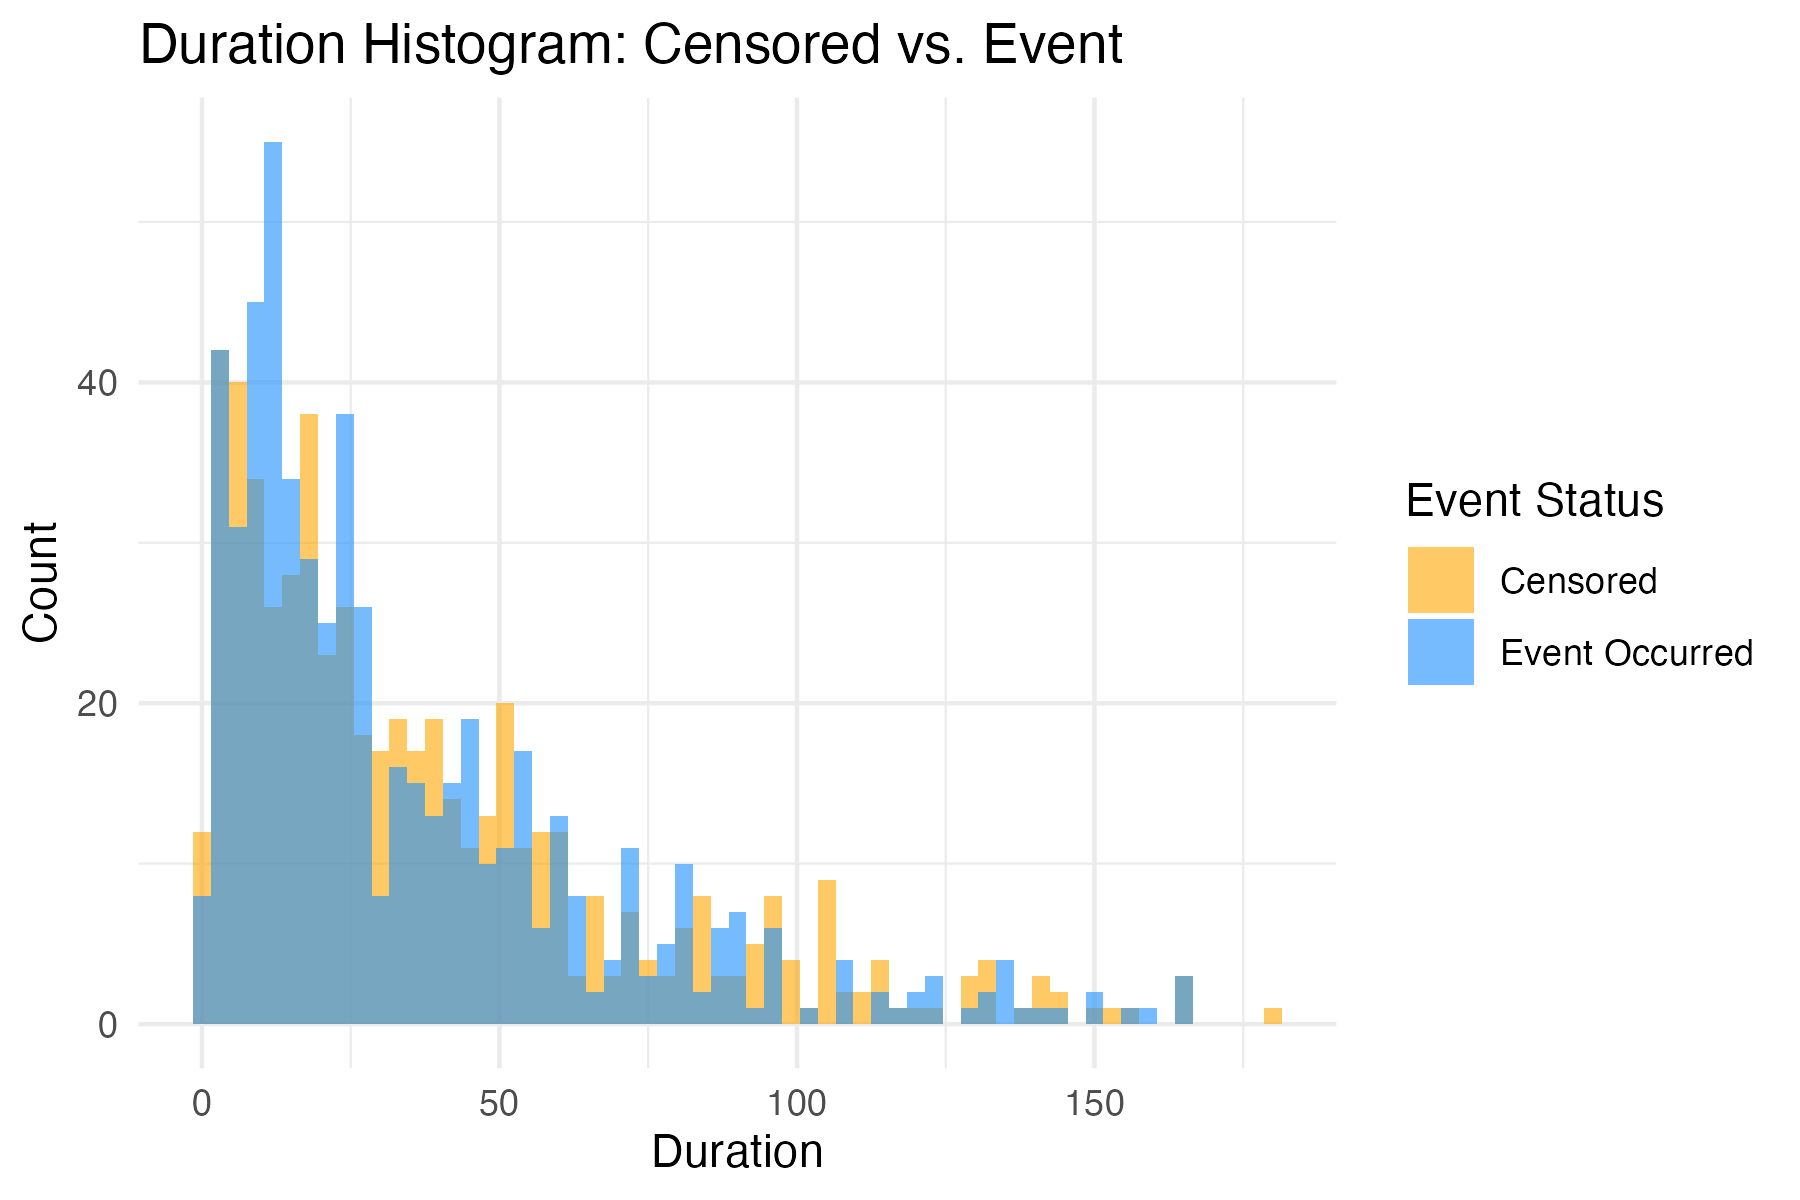
\includegraphics[height=5.5cm, width=0.6\textwidth]{images/separate_hist.png}
    \caption{{\small Histograms of censored and event durations in the employee turnover data}}
    \label{fig:离职数据分开的直方图}
\end{figure}
To illustrate the effect of unrealistic observation windows, we simulate under two settings, $A = 30$ and $A = 1000$, and plot the empirical cumulative distribution functions (ECDFs) for both the event subsample ($\delta = 1$) and the censored subsample ($\delta = 0$), along with the histograms of simulated durations.
\begin{itemize}
    \item $A = 30$ (Figure~\ref{fig:ppc-A30}). Relative to the real-data histogram (Figure~\ref{fig:离职数据分开的直方图}), simulated durations are tightly compressed within 0–30 months, with both events and censorings occurring unusually early. The ECDFs (Figure~\ref{fig:ecdf-event_a30}, red lines) rise sharply at short durations and diverge from the observed curves, highlighting the impact of an unrealistically small $A$ rather than any misfit in the event-time parameter $\lambda$.
    \item $A = 1000$ (Figure~\ref{fig:ppc-A1000}). The simulated histogram in Figure~\ref{fig:fake-hist_a1000} shows durations that are widely dispersed, and the ECDF curves (Figure~\ref{fig:ecdf-event_a1000}, red lines) align more closely with the observed data than in the $A=30$ case. However, when compared with the real-data histogram in Figure~\ref{fig:离职数据分开的直方图}, this setting implies a maximum tenure approaching 83 years—far beyond any realistic employment scenario. The apparent visual agreement is therefore driven by an implausible survey window rather than by an accurate recovery of the event-time distribution, making such a setting unsuitable for credible model checking.
\end{itemize}
\begin{figure}[H]
\centering
\begin{subfigure}[t]{0.64\textwidth}
  \centering
  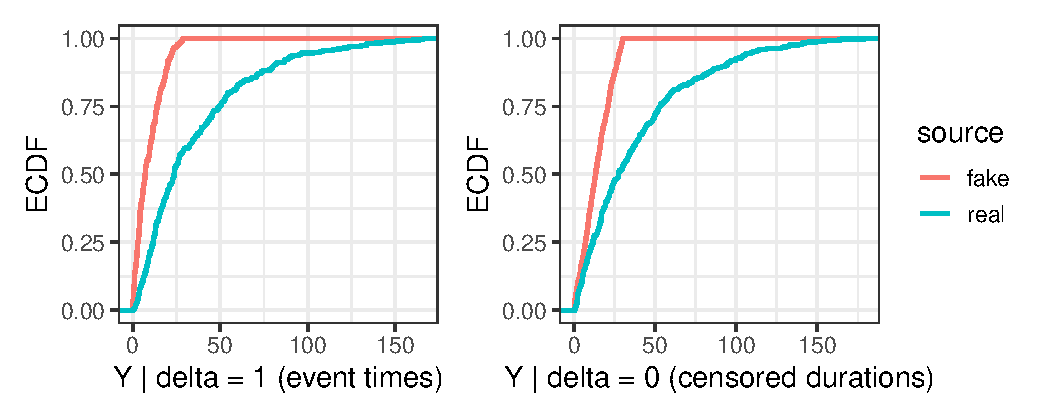
\includegraphics[height=4.5cm, width=\textwidth]{images/ppc_two_a30.pdf}  % 图1路径
  \caption{{\small ECDFs}}
  \label{fig:ecdf-event_a30}
\end{subfigure}
\begin{subfigure}[t]{0.351\textwidth}
  \centering
  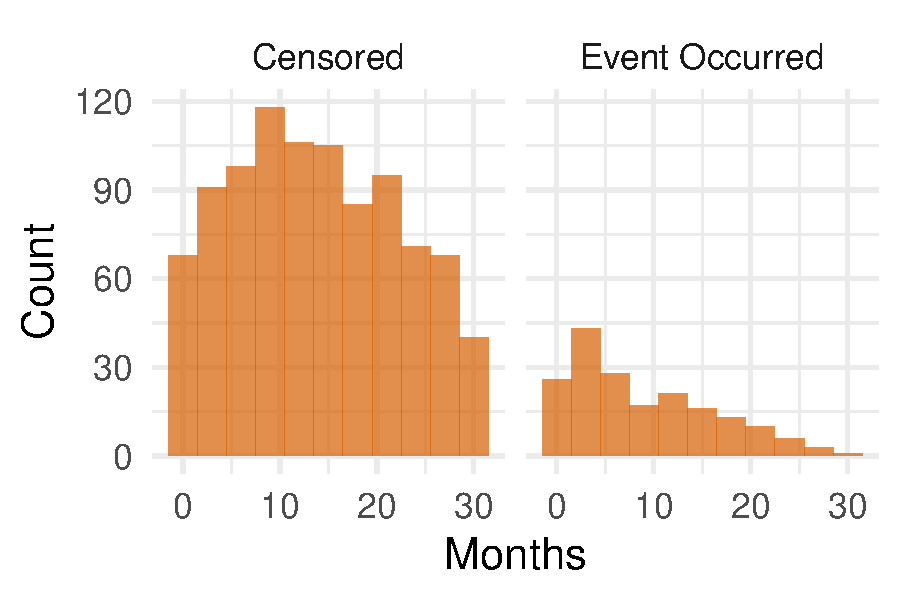
\includegraphics[height=4.5cm,width=\linewidth]{images/fake_duration_hist_a30.pdf}   % 图3路径
  \caption{{\small Fake-data histogram}}
  \label{fig:fake-hist_a30}
\end{subfigure}
\caption{{\small Posterior predictive checking ($A=30$).}}
\label{fig:ppc-A30}
\end{figure}
%%%%%%%%%%%%%%%%%%%%%%
\begin{figure}[H]
\centering
\begin{subfigure}[t]{0.64\textwidth}
  \centering
  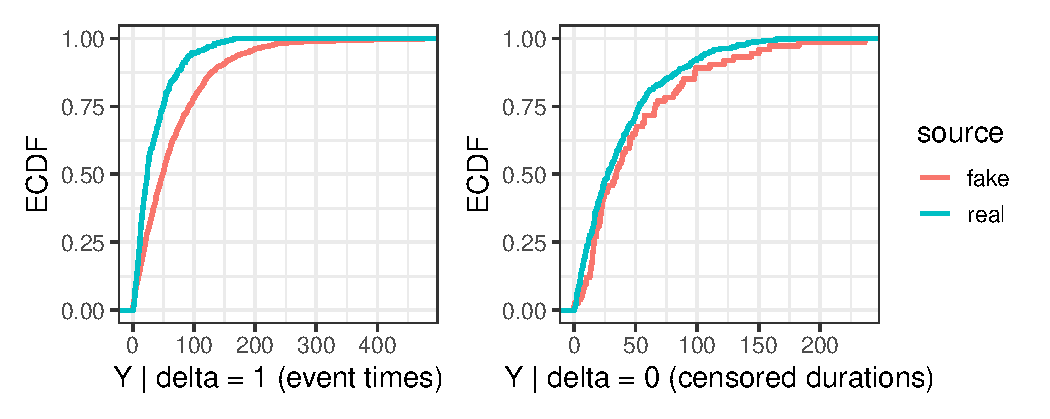
\includegraphics[height=4.5cm,width=\textwidth]{images/ppc_two_a1000.pdf}  % 图1路径
  \caption{{\small ECDFs}}
  \label{fig:ecdf-event_a1000}
\end{subfigure}
\begin{subfigure}[t]{0.351\textwidth}
  \centering
  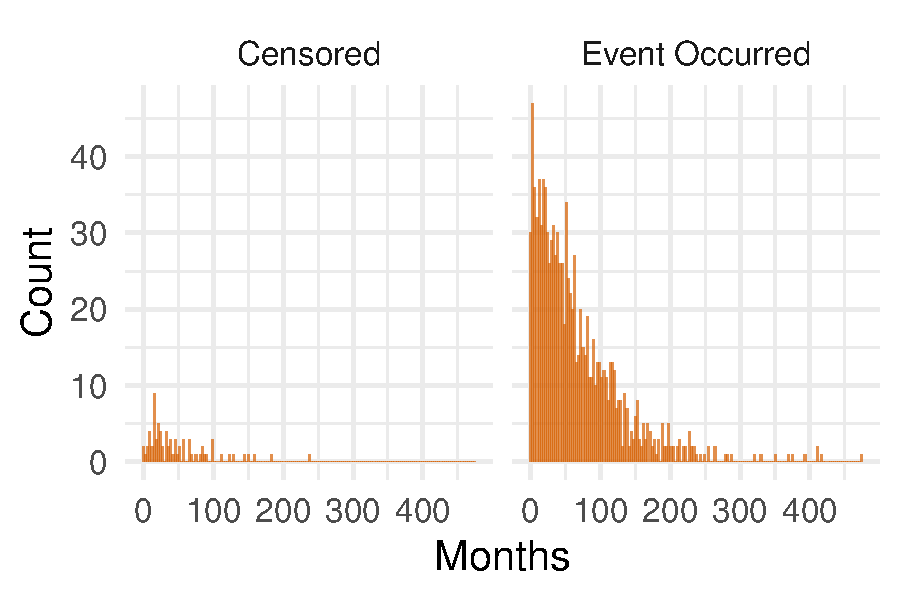
\includegraphics[height=4.5cm,width=\linewidth]{images/fake_duration_hist_a1000.pdf}   % 图3路径
  \caption{{\small Fake-data histogram}}
  \label{fig:fake-hist_a1000}
\end{subfigure}
\caption{{\small Posterior predictive checking ($A=1000$).}}
\label{fig:ppc-A1000}
\end{figure}
These examples underscore that posterior predictive fit must be interpreted in light of the plausibility of data-generating assumptions. Determining a realistic range for $A$ is essential for credible model checking, and this motivates the next step—explicitly incorporating $A$ into the likelihood and estimating it jointly with event-time parameters.